\section{Google Maps API}\label{sec:googlemapsapi}
The Google Maps API \citep{misc:googlemapsapi} is used to show the map on both the front page and the admin page.
However, both of these pages use the API differently, the front page uses the API to show the map with the stations that are currently in the system, whereas the admin page visualises where all the bicycles are located.

To use the API, the construction of the map is done first, which can be seen in \lstref{lst:mapoptions}.
Map options are chosen here, these options are e.g. the center of the map, which zoom level the map should have, and the style of the map.

\begin{minipage}{\textwidth}
\begin{lstlisting}[caption={Construction of the map}, label={lst:mapoptions}, language=Javascript]
var mapOptions = {
	zoom: 13,
	center: aalborg,
	panControl: false,
    zoomControlOptions: {
		style: google.maps.ZoomControlStyle.LARGE,
		position: google.maps.ControlPosition.RIGHT_TOP,
	}
};
\end{lstlisting}
\end{minipage}

After the map is constructed the map is filled with either the stations or the bicycles, depending on the page.

For the front page the stations are inserted into the map by use of AJAX.
For each station, the work-flow of this is as follows:

\begin{description}[style=nextline]
	\item[Gather data]
	Use the stationservice to read data to be displayed on map.
	\item[Create info window]
	The info window is a window that appears whenever the user clicks on a station marker.
	The info window shows information about the station, which is the name, amount of free bicycles, and the amount of free docks.
	\item[Marker creation]
	Create a marker, which are the bulletpoints indicating the station on the map.
	The creation of the marker contains position, title, icon.
	\item[Assign listeners]
	Assign listeners to the marker clicks, in order to show the infowindow for the given marker when the marker is clicked.
\end{description}

\begin{figure}[h]
	\centering
	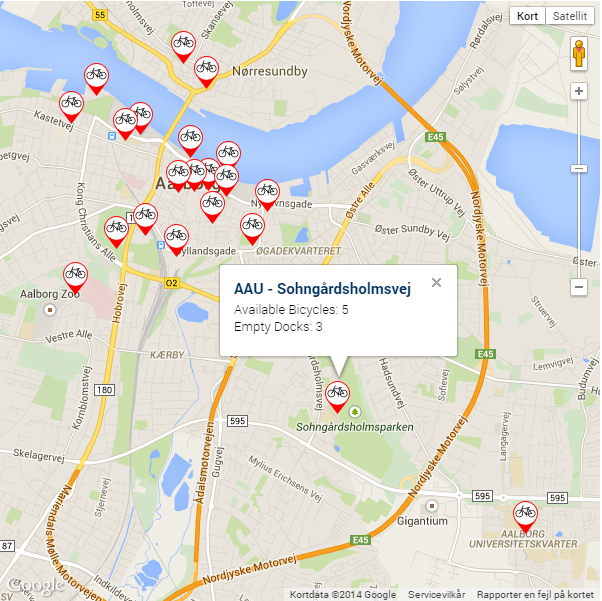
\includegraphics[scale=0.7]{googlemarkermap}
	\caption{Google map with station markers and info window shown}
	\label{fig:googlemapmarkerinfowindow}
\end{figure}

An example of the final google map with markers placed can be seen in \figref{fig:googlemapmarkerinfowindow}.

For the admin page the markers are bicycles, which are updated at a set frequency using AJAX, and is created in a similar fashion, just by other objects placed on the map.
The main purpose of the admin tracking page is to be able to see where the different bicycles are at a given time, which is the reason why the markers are updated once in a while.
For the purpose of this project it updates every tenth second, to be able to simulate how it could look like, however, in the real system every tenth second might be too often, depending on how often the GPS's of the bicycle send data to the database.
For the update of the marker position AJAX is used to get all the positions of the different bicycles, which allows the makers to move without refreshing the page.